\documentclass{article}
\usepackage[utf8]{inputenc}
\usepackage[margin=1in]{geometry}
\usepackage[colorlinks=true,
            linkcolor=red,
            urlcolor=blue,
            citecolor=red]{hyperref}
\usepackage{booktabs}
\usepackage{color}
\usepackage{graphicx}
\usepackage{float}
\usepackage{multirow}
\usepackage{multicol}
\usepackage{amsmath}
\usepackage{graphicx}
\graphicspath{ {./figures/} }
\newcommand{\yueran}[1]{{\color{red}[Yueran: #1]}}
\newcommand{\zongyuan}[1]{{\color{blue}[Zongyuan: #1]}}

\title{\vspace{-1.5cm}5741 Project Midterm Report: H-1B Petition Analysis}
\author{Yueran Yang (yy595), Zongyuan Yuan (zy225)}
\date{}

\begin{document}
\maketitle
\vspace{-3em}

\section{Problem Statement}
The Labor Condition Application (LCA) is an application for the employer to hire a foreign worker in a specific position for no more than 3 years. H-1B Lottery is followed by approval of LCA. This project is aimed at predicting the case status of an LCA application based on the relevant information of a foreign employee in a company such as wage, job type, etc.

\section{Dataset}
\begin{multicols}{2}
\subsection{About the Dataset}
The raw data contains 2,448,729 rows and 36 columns. All features and counts of NA entry for each feature is shown in Table \ref{data_intro} in Appendix \ref{data_intro_sec}. 

SOC\_CODE refers to Standard Occupation Classification, which is to classify workers into  categories.\footnote{See \url{https://www.bls.gov/soc/}} In this project, we use 2010 SOC System\footnote{See \url{https://www.bls.gov/soc/2010/2010\_major\_groups.htm}}. NAIC refers to North American Industry Classification. NAIC\_CODE is used to classify the business of a company \footnote{See \url{https://www.census.gov/naics/}}. 

CASE\_STATUS is the label in our project. It contains four status, CERTIFIED, WITHDRAWN, DENIED and CERTIFIED-WITHDRAWN. Thus, the goal of the project is to solve a multi-class classification problem. 

\subsection{Data Processing}
After deleting all redundant features shown in Table \ref{data_intro}. We first remove all the rows that contain NA. We do not consider fill in the values because the number of rows containing NA is quite small as shown in the table and it is hard to use any method to fill in those critical information. Similarly, if there are invalid values in the following cleaning process, we simply delete the samples. 

For NAIC\_CODE, we only keep 4 digits. The length of the code can be 2 to 6. The longer the code, the more detailed the classification. If we keep the original data, there will be 531 different values in this categorical feature, which can be too detailed for training and may cause over-fitting. Thus, we only consider to keep 3 digits with 190 different values. 

For SOC\_CODE, similar to NAIC\_CODE, we only keep 3 digits, which decrease the number of different values from 1238 to 100. 

For Date features (EMPLOYER\_START\_DATE, EMPLOYER\_END\_DATE, CASE\_SUBMITTED and DECISION\_DATE), we use the duration as the new features and delete the original four features. For wages, we use the units of pay and values of wage to calculate the yearly wage as our feature. 

For EMPLOYER\_NAME, we count the frequency of a company in the data set and estimate the possibility of the four status for a specific company as the prior possibility.

For other categorical feature, we use one-hot vectors. The final data contains 422 columns and 2435102 rows. 

\subsection{EDA}

We first look at the distribution of CASE\_STATUS. From the bar plot below, we can see that most of the applications are certified. 

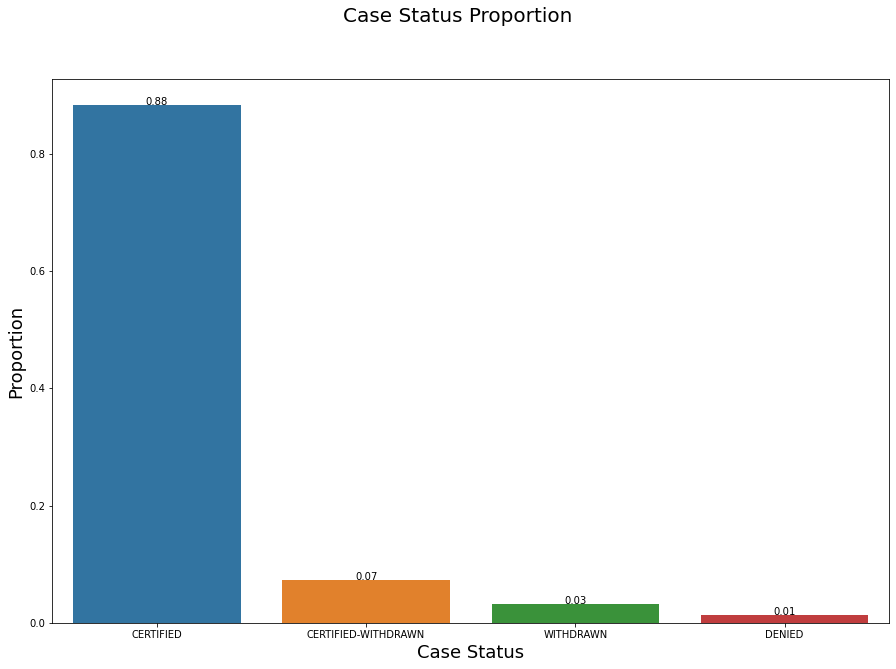
\includegraphics[scale=0.25]{figures/fig11.png}

Therefore, the labels of our data set is very unbalanced. 

As we looked at the dataset, we found that there are 169,810 companies that submitted applications. If we were to use one-hot encoding for the feature EMPLOYER\_NAME, the dimension of our dataset would be too large to handle. Therefore, we want to keep only a subset of companies that that contributed a large proportion of total applications. The following histogram shows the top 50 companies that submitted most applications.

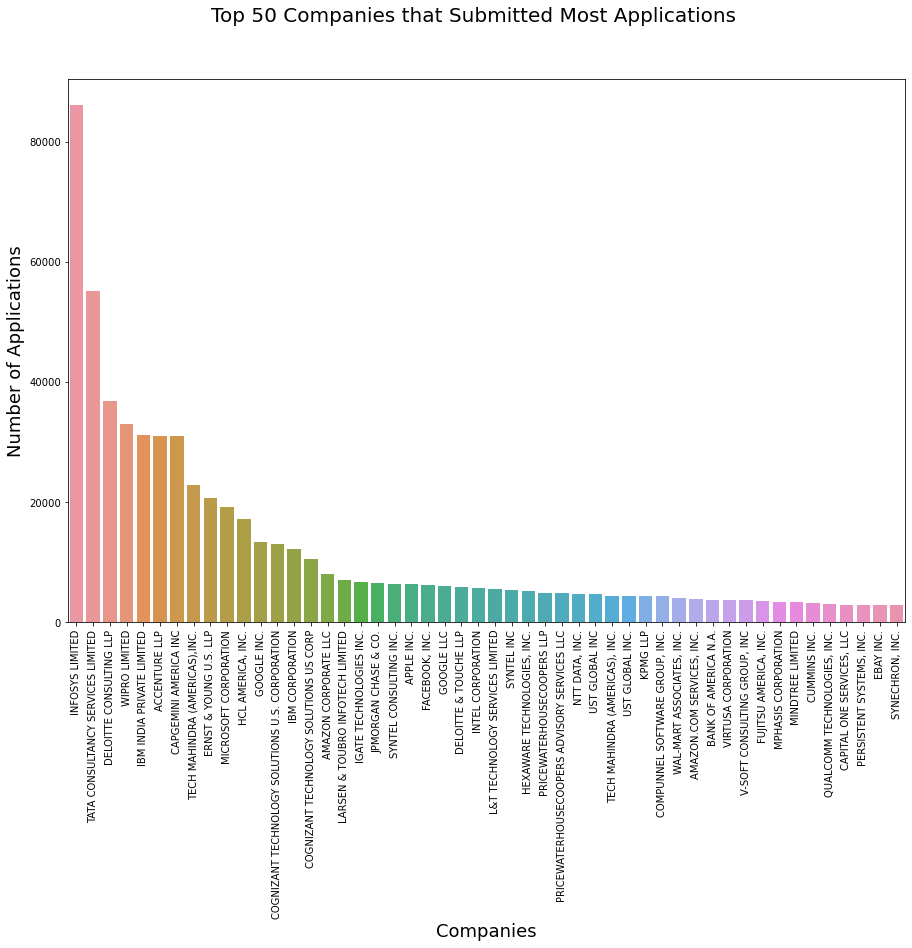
\includegraphics[scale=0.24]{figures/fig7.png}

Another important factor is the location of the employer. From the plot below, we can see that the applications from employers in some states are more likely to be certified than others.



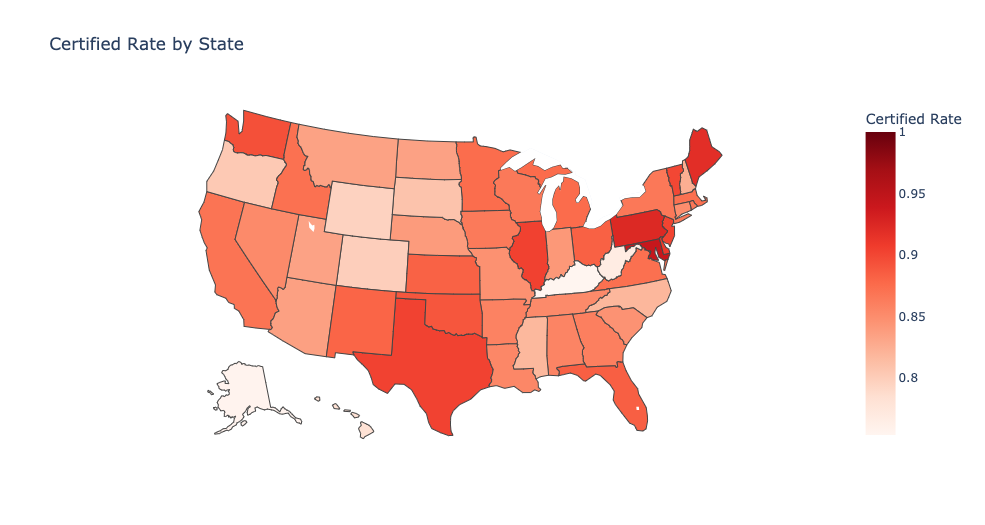
\includegraphics[scale=0.24]{figures/fig3.png}

Wage is an important indicator of the value of the job. Empirically, the higher the wage, the more likely an application might be certified. The violin plot below shows that average wages in certified applications are slightly higher than average wages in applications with other status.

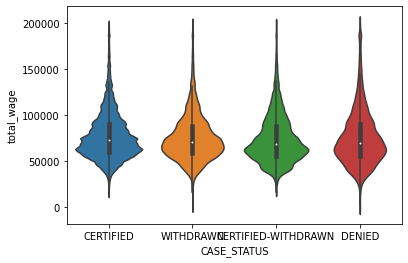
\includegraphics[scale=0.5]{figures/wage_violin.png}

From the wage distribution below, we can see that most applications have wages from 50,000 to 100,000.

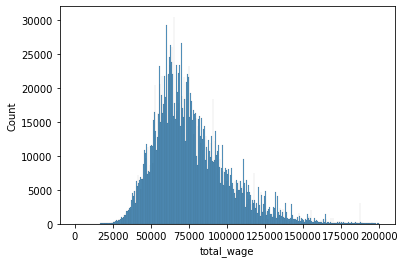
\includegraphics[scale=0.5]{figures/wage_hist.png}

The majority of the applications have SOC code that starts with 15 meaning that most of the applications are computer or software related.

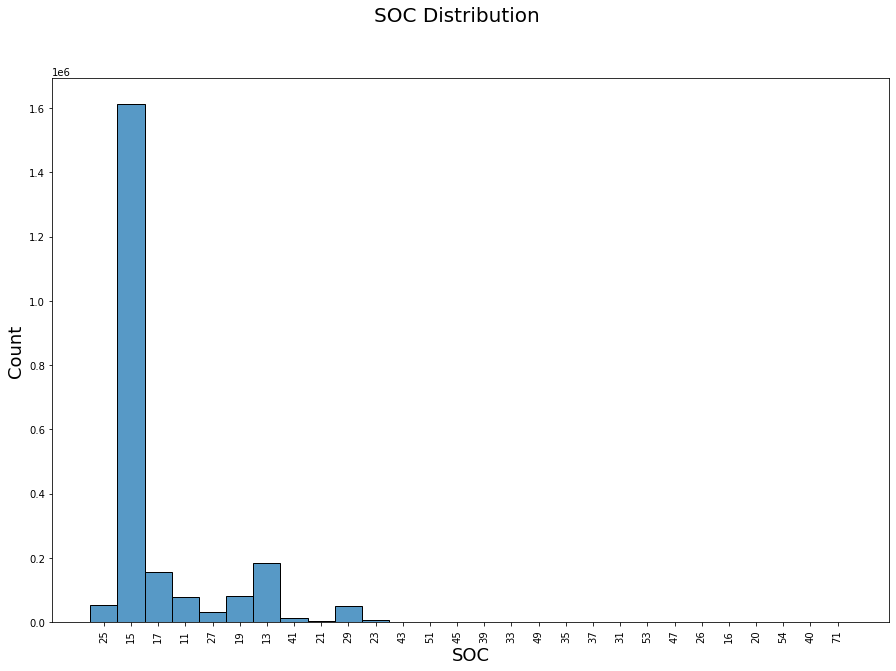
\includegraphics[scale=0.25]{figures/fig8.png}
% \usepackage{multirow}
% \usepackage{graphicx}
\begin{table*}[ht]
\centering
\caption{F1-Score for Each Label} 
\label{table: perform}
\resizebox{\textwidth}{!}{%
\begin{tabular}{|c|cccc|}
\hline
\multirow{2}{*}{\textbf{Model}} & \multicolumn{4}{c|}{\textbf{TEST F1-Score}}                                                                                                            \\ \cline{2-5} 
                                & \multicolumn{1}{c|}{\textbf{CERTIFIED}} & \multicolumn{1}{c|}{\textbf{CERTIFIED-WITHDRAWN}} & \multicolumn{1}{c|}{\textbf{WITHDRWN}} & \textbf{DENIED} \\ \hline
Decision Tree                   & \multicolumn{1}{c|}{0.9900}             & \multicolumn{1}{c|}{0.9343}                       & \multicolumn{1}{c|}{0.7452}            & 0.0000          \\ \hline
Logistic Regression             & \multicolumn{1}{c|}{0.9708}             & \multicolumn{1}{c|}{0.8611}                       & \multicolumn{1}{c|}{0.1903}            & 0.4034          \\ \hline
LDA                             & \multicolumn{1}{c|}{0.9559}             & \multicolumn{1}{c|}{0.6993}                       & \multicolumn{1}{c|}{0.2735}            & 0.4635          \\ \hline
\multirow{2}{*}{\textbf{Model}} & \multicolumn{4}{c|}{\textbf{TRAINING F1-Score}}                                                                                                        \\ \cline{2-5} 
                                & \multicolumn{1}{c|}{\textbf{CERTIFIED}} & \multicolumn{1}{c|}{\textbf{CERTIFIED-WITHDRAWN}} & \multicolumn{1}{c|}{\textbf{WITHDRWN}} & \textbf{DENIED} \\ \hline
Decision Tree                   & \multicolumn{1}{c|}{0.9898}             & \multicolumn{1}{c|}{0.9327}                       & \multicolumn{1}{c|}{0.7412}            & 0.0000          \\ \hline
Logistic Regression             & \multicolumn{1}{c|}{0.9707}             & \multicolumn{1}{c|}{0.8570}                       & \multicolumn{1}{c|}{0.1897}            & 0.4065          \\ \hline
LDA                             & \multicolumn{1}{c|}{0.9560}             & \multicolumn{1}{c|}{0.6941}                       & \multicolumn{1}{c|}{0.2757}            & 0.4611          \\ \hline
\end{tabular}%
}
\end{table*}



\section{Preliminary Models}
\iffalse
\yueran{\url{https://analyticsindiamag.com/7-types-classification-algorithms/}}

\noindent\yueran{\url{https://scikit-learn.org/stable/modules/multiclass.html}}

\noindent\yueran{\url{https://www.datascienceblog.net/post/machine-learning/performance-measures-multi-class-problems/}}

\noindent\yueran{SOC\_CODE:\url{https://www.bls.gov/soc/2010/2010\_major\_groups.htm}}
\fi
We developed three preliminary models: 1. Decision tree with two levels 2. Logistic Regression 3. Linear Discriminant Analysis (LDA)

\subsection{Performance of the Three Models}
Since the labels of the dataset is very unbalanced, using accuracy as our metric is not reflective of the model performance. Therefore, we use F1 score instead. F1 is defined as follows: $$ \frac{2\times(precision \times recall)}{precision + recall}$$
where precision is defined as $$\frac{\text{TRUE POSITIVE}}{\text{TRUE POSITIVE} + \text{FALSE POSITIVE}}$$ and recall is defined as $$\frac{\text{TRUE POSITIVE}}{\text{TRUE POSITIVE} + \text{FALSE NEGATIVE}}_.$$

Table \ref{table: perform} summarizes the performance of the three models using F1 Score.

\subsection{Model Performance Analysis} 

\hspace{1.5em}\textbf{Decision Tree}

We set the maximum depth of decision tree to 2 because our dataset is very large. Setting the max depth more than 2 is too computationally demanding.

\textbf{Logistic Regression}

Logistic Regression for muilt-class classification is to train as many models as as the distinct labels and output the label with the largest possibility. In our case, the model trained four binary logistic models for each label. In the preliminary model, we use logistic regression with no regularization and no weight on training. The training process using Logistic Regression in sklearn is quite slow (about 5 hours) on our training sets. 

\textbf{LDA}

The main idea of LDA is to train distinct models using data with the same label and to calculate $P(Y = k| X = x)$ using Bayes Theorem. The output is $\arg\max_{k \in K} P(Y = k| X = x)$. The method is expected to have more balanced performance on each label, which can be inferred from Table \ref{table: perform}. 

\textbf{Conclusion}

All three models have bad performance on cases that are denied. This is because data with denied labels constitute only around 1 percent of the entire dataset. 

\section{Further Steps}
There are several problems after pre-processing and preliminary model. 
\begin{itemize}
    \item The one-hot vectors for each categorical feature are too sparse and may contain redundant features, causing the data set to be too large to try some complicated models by using sklearn. Even reading the data into python would need 2.5 minutes. The jupyter notebook kernals always fail due to RAM limit when fitting a model. 
    \item For this muilt-class classification problem, we need to find a reasonable way to measure the performance of models on the whole dataset instead of using the measurement for each class separately. 
    \item Though the total accuracy is very high, the accuracy for each label is quite different, and the predictions on WITHDRAWN and DENIED are especially terrible. It is mainly because that the data set is imbalanced on each label. The CERTIFIED labels account for over 90\% of the total labels. 
\end{itemize}
Thus, our further steps would be around feature selections and further improve our models on imbalanced dataset. We may include weights in different classes or use other ways to boost our data  in the training. For the feature selection, we are planning to use PCA for reducing dimension of the features while preserving as much important information as we can and use regularization for feature selections. Also, to solve the problem on RAM limit crash, we would apply spark (pyspark in python) to train those models.
\end{multicols}
\newpage
\section{Appendix}
\subsection{Data Intro} \label{data_intro_sec}

\begin{table}[H]
\centering
\caption{Counts of NA for each feature}
\label{data_intro}
\begin{tabular}{lll}
\hline
Name & NACount & Note\\ \hline
Sector\_data & 2 & {\color{red}Delete }\\ \hline
EMP\_STATE\_full & 2358 & {\color{red}Delete }\\ \hline
EMP\_State\_and\_city & 0 & {\color{red}Delete }\\ \hline
Worksite\_STATE\_full & 2453 & {\color{red}Delete }\\ \hline
Worksite\_State\_and\_city & 0 & {\color{red}Delete }\\ \hline
EMPLOYER\_PHONE & 1 & {\color{red}Delete }\\ \hline
AGENT\_ATTORNEY\_NAME & 227034 & {\color{red}Delete }\\ \hline
AGENT\_ATTORNEY\_CITY & 840452 & {\color{red}Delete }\\ \hline
AGENT\_ATTORNEY\_STATE & 899957 & {\color{red}Delete }\\ \hline
JOB\_TITLE & 11 & {\color{red}Delete }\\ \hline
EMPLOYER\_POSTAL\_CODE & 57 & {\color{red}Delete }\\ \hline
WORKSITE\_POSTAL\_CODE & 70 & {\color{red}Delete }\\ \hline
YEAR & 0 & {\color{red}Delete }\\ \hline
WORKSITE\_COUNTY & 4616 & {\color{red}Delete }\\ \hline
WORKSITE\_CITY & 41 & {\color{red}Delete }\\ \hline
WAGE\_RATE\_OF\_PAY & 0 & {\color{red}Delete }\\\hline
SOC\_NAME & 20 & {\color{red}Delete }\\ \hline
EMPLOYER\_CITY & 29 & {\color{red}Delete }\\ \hline
CASE\_NUMBER & 0 & {\color{red}Delete }\\ \hline
CASE\_STATUS & 0 & {\color{green}label }\\ \hline
CASE\_SUBMITTED & 1 &  {\color{blue} calculate duration }\\ \hline
DECISION\_DATE & 0 & {\color{blue} calculate duration }\\ \hline
EMPLOYMENT\_START\_DATE & 38 & {\color{blue} calculate duration }\\ \hline
EMPLOYMENT\_END\_DATE & 47 & {\color{blue} calculate duration }\\ \hline
EMPLOYER\_COUNTRY & 0 & {\color{blue} Only consider America. }\\ \hline
PREVAILING\_WAGE & 0 & {\color{blue} Normalize it to yearly wage. }\\ \hline
PW\_UNIT\_OF\_PAY & 0 & {\color{blue} Normalize it to yearly wage. }\\ \hline
WAGE\_UNIT\_OF\_PAY & 19 & {\color{blue} Normalize it to yearly wage. }\\ \hline
total\_wage & 0 & {\color{blue} Normalize it to yearly wage. }\\ \hline
NAIC\_CODE & 2 & {\color{blue} Keep three digits. }\\ \hline
EMP\_STATE\_abb & 0 & {\color{blue} For geographical figures. }\\ \hline
SOC\_CODE & 18 & {\color{blue} Keep three digits. }\\ \hline
EMPLOYER\_NAME & 67 & {\color{blue} Count frequency }\\ \hline
VISA\_CLASS & 0 & \\ \hline
FULL\_TIME\_POSITION & 7 & \\ \hline
Worksite\_STATE\_abb & 16 & \\ \hline
\end{tabular}
\end{table}

\end{document}
